\renewcommand*{\arraystretch}{1.1}

\subsection*{Interactive / complex / 7}
\label{section:interactive-complex-read-07}

% change \emph{} to use sans-serif font
\let\oldemph\emph
\renewcommand{\emph}[1]{{\footnotesize \sf #1}}

\renewcommand{\currentQueryCard}{7}
\marginpar{
	\raggedleft
	\vspace{0.22ex}

	\queryRefCard{interactive-complex-read-01}{IC}{1}\\
	\queryRefCard{interactive-complex-read-02}{IC}{2}\\
	\queryRefCard{interactive-complex-read-03}{IC}{3}\\
	\queryRefCard{interactive-complex-read-04}{IC}{4}\\
	\queryRefCard{interactive-complex-read-05}{IC}{5}\\
	\queryRefCard{interactive-complex-read-06}{IC}{6}\\
	\queryRefCard{interactive-complex-read-07}{IC}{7}\\
	\queryRefCard{interactive-complex-read-08}{IC}{8}\\
	\queryRefCard{interactive-complex-read-09}{IC}{9}\\
	\queryRefCard{interactive-complex-read-10}{IC}{10}\\
	\queryRefCard{interactive-complex-read-11}{IC}{11}\\
	\queryRefCard{interactive-complex-read-12}{IC}{12}\\
	\queryRefCard{interactive-complex-read-13}{IC}{13}\\
	\queryRefCard{interactive-complex-read-14}{IC}{14}\\
}


\noindent\begin{tabularx}{\queryCardWidth}{|>{\queryPropertyCell}p{\queryPropertyCellWidth}|X|}
	\hline
	query & Interactive / complex / 7 \\ \hline
%
	title & Recent likers \\ \hline
%
	pattern & \centering 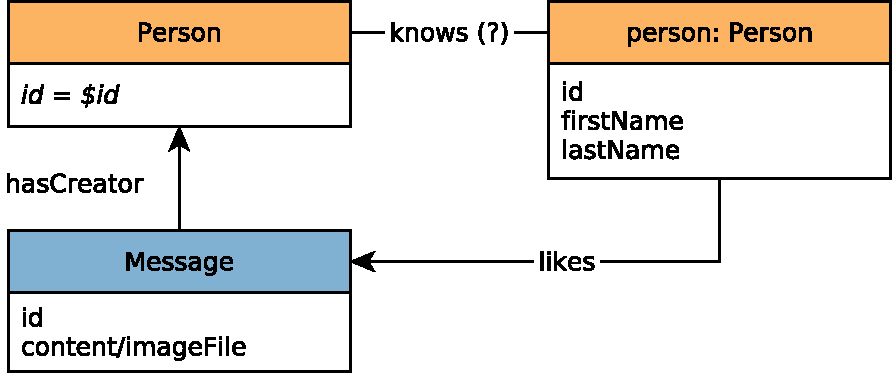
\includegraphics[scale=\patternscale,margin=0cm .2cm]{patterns/interactive-complex-read-07} \tabularnewline \hline
%
	desc. & Given a start \emph{Person}, find (most recent) \texttt{likes} on any of
start \emph{Person}'s \emph{Messages}. Find \emph{Persons} that liked
(\texttt{likes} edge) any of start \emph{Person}'s \emph{Messages}, the
\emph{Messages} they liked most recently, the creation date of that
like, and the latency in minutes (\texttt{minutesLatency}) between
creation of \emph{Messages} and like. Additionally, for each
\emph{Person} found return a flag indicating (\texttt{isNew}) whether
the liker is a friend of start \emph{Person}. In case that a
\emph{Person} liked multiple \emph{Messages} at the same time, return
the \emph{Message} with lowest identifier.
 \\ \hline
%
	
		params &
		\innerCardVSpace{\begin{tabularx}{\attributeCardWidth}{|>{\paramNumberCell}c|>{\varNameCell}M|>{\typeCell}m{\typeWidth}|Y|} \hline
		$\mathsf{1}$ & Person.id
 & 64-bit Integer
 & \texttt{personId}
 \\ \hline
		\end{tabularx}}\innerCardVSpace \\ \hline
	
%
	
		result &
		\innerCardVSpace{\begin{tabularx}{\attributeCardWidth}{|>{\resultNumberCell}c|>{\varNameCell}M|>{\typeCell}m{\typeWidth}|>{\resultOriginCell}c|Y|} \hline
		$\mathsf{1}$ & Person.id & ID & R &
				\texttt{personId}
 \\ \hline
		$\mathsf{2}$ & Person.firstName & String & R &
				\texttt{personFirstName}
 \\ \hline
		$\mathsf{3}$ & Person.lastName & String & R &
				\texttt{personLastName}
 \\ \hline
		$\mathsf{4}$ & Like.creationDate & DateTime & R &
				\texttt{likeCreationDate}
 \\ \hline
		$\mathsf{5}$ & Message.id & ID & R &
				\texttt{commentOrPostId}
 \\ \hline
		$\mathsf{6}$ & Message.content or Post.imageFile & String & R &
				\texttt{commentOrPostContent}
 \\ \hline
		$\mathsf{7}$ & minutesLatency & 32-bit Integer & C &
				\texttt{minutesLatency} -- Duration between creation of the
\emph{Message} and the creation of the like, in minutes
 \\ \hline
		$\mathsf{8}$ & isNew & Boolean & C &
				\texttt{isNew} -- \texttt{false} if liker \emph{Person} is friend of
start \emph{Person}, \texttt{true} otherwise
 \\ \hline
		\end{tabularx}}\innerCardVSpace \\ \hline
	
%
	
		sort		&
		\innerCardVSpace{\begin{tabularx}{\attributeCardWidth}{|>{\sortNumberCell}c|>{\varNameCell}M|>{\directionCell}c|Y|} \hline
		$\mathsf{1}$ & Like.creationDate
 & $\desc
$ &  \\ \hline
		$\mathsf{2}$ & Person.id
 & $\asc
$ &  \\ \hline
		\end{tabularx}}\innerCardVSpace \\ \hline
	%
	limit & 20 \\ \hline
	%
	CPs &
	\multicolumn{1}{>{\raggedright}l|}{
		\chokePoint{2.2}, 
		\chokePoint{2.3}, 
		\chokePoint{3.3}, 
		\chokePoint{5.1}, 
		\chokePoint{8.1}, 
		\chokePoint{8.3}
		} \\ \hline
	%
	relevance &
		\footnotesize This query looks for paths of length two, starting from a given
\emph{Person}, moving to its published messages and then to
\emph{Persons} who liked them. It tests several aspects related to join
optimization, both at query optimization plan level and execution engine
level. On the one hand, many of the columns needed for the projection
are only needed in the last stages of the query, so the optimizer is
expected to delay the projection until the end. This query implies
accessing two-hop data, and as a consequence, index accesses are
expected to be scattered. We expect to observe variate cardinalities,
depending on the characteristics of the input parameter, so properly
selecting the join operators will be crucial. This query has a lot of
correlated sub-queries, so it is testing the ability to flatten the
query execution plans.
 \\ \hline%
\end{tabularx}
\queryCardVSpace

% change \emph back to the old one
\let\emph\oldemph